\documentclass[UTF8]{ctexart}

\usepackage[
  backend=biber,
  style=gb7714-2015,
  gbnamefmt=givenahead
]{biblatex}
\addbibresource{wenxian.bib}

\usepackage{amsmath}
\usepackage{subcaption}
\usepackage{graphicx}
\usepackage{caption}
\usepackage{txfonts}
\usepackage{hyperref}
\usepackage[T1]{fontenc}

\usepackage{authblk}
\usepackage{indentfirst}
\setlength{\parindent}{2em}
\usepackage[a4paper, top=3cm, bottom=2.5cm, left=2cm, right=2cm]{geometry}

\usepackage{fancyhdr}
\pagestyle{fancy}
\fancyhf{}
\fancyfoot[C]{\thepage}
\renewcommand{\headrulewidth}{0pt}

% ===== 行距设置：接近 Word 1.5 倍 =====
\usepackage{setspace}
\setstretch{1.5}

% ===== 字体设置 =====
\setCJKmainfont{SimSun}
\setCJKsansfont{SimHei}

\usepackage{float}
\usepackage{array}
\usepackage{tabularx}
\usepackage{booktabs}
\usepackage{enumitem}
\usepackage{xurl}

\graphicspath{{images/}}
\captionsetup{font=small}
\renewcommand{\arraystretch}{1.25}
\setlength{\tabcolsep}{6pt}
\setlist[enumerate]{itemsep=0.2em, topsep=0.2em, parsep=0pt, partopsep=0pt}

\newcolumntype{Y}{>{\raggedright\arraybackslash}X}

\begin{document}

\begin{center}
  {\heiti\zihao{2} 立项依据\par}
\end{center}
\vspace{1em}

\section*{（一）项目简介}

本项目拟建设“湘言通”湖南方言与普通话双向转换及开放语料数据库平台，以湖南地区方言资源的数字化整理、规范化存储与共享应用为主要研究目标，围绕“方言资源库建设”和“方言转换服务实现”两方面展开研究与实践。项目依托现有网页原型\url{https://thisshy.github.io/hunan-mandarin-converter/}，在既有功能基础上，进一步完善数据采集、人工审核、结构化入库、双向转换、共享下载、场景适配和移动端延展等环节，逐步建成一个兼顾研究、展示与应用的方言数字平台。平台的服务对象不只包括普通用户，也包括方言学习者、地方文化传播工作者、相关研究人员以及后续可能接入本项目数据的开发者。换句话说，本项目既要解决资源保存的问题，也要回应资源如何被看见、被使用、被继续补充的问题。

近年来，国家持续推进语言文字信息化建设、文化资源数字化建设和语言资源保护工程，明确提出要加强数字中文建设，提升语言资源的数字化水平和服务能力\cite{jiaoyubu2025shuzi,quanguorenda2000putonghua,zhongxuan2022wenhua,zhonggong2023shuzi,jiaoyubu2024baohu}。这说明，方言资源的整理、保存与应用，已经不再只是传统语言调查中的附属工作，而是与数字中国建设、文化数字化战略以及国家语言资源保护工作紧密相关。对于高校项目而言，这类选题也有比较清楚的实践空间：一方面可以借助学生团队完成资料整理、平台搭建和样本采集，另一方面又能够把地方文化资源转化为长期可用的数字成果，而不是停留在一次性的展示活动中。

湖南方言中大量词汇、句式和口语表达，至今仍分散于个体记忆、地方口述材料、网络文本、日常交流以及专业词典、地方语言研究书籍等资料之中，缺乏统一、规范且可持续更新的整理机制。现有材料来源零散、字段不统一，地区标注、语义说明、适用场景等信息往往缺失，难以沉淀为可长期使用的公共资源。有些表达在不同地区意思接近，用词却并不一致；有些词汇只在特定语境中成立，脱离上下文便容易误读。普通用户、方言学习者、研究人员和开发者，在理解、检索、转换和比对方言时又普遍存在现实需求，但现有工具大多停留在静态展示或零散查询层面，缺少以数据库为支撑、以服务为导向的综合平台。

因此，本项目并非仅仅制作一个简单的网页原型，而是希望在数据库建设的基础上，逐步形成“数据采集—人工审核—资源入库—双向转换—评测反馈—后续拓展”的完整工作链条。这个链条的价值在于，前端展示、后台管理和数据积累不是彼此割裂的几个模块，而是围绕同一套方言资源持续运转。通过这一平台，可以在方言资源保护、方言数字化服务与地方文化传播之间建立起较为清晰的联系，也能为后续的语音扩展、教学使用和地方文化展示保留接口。当前 APP 原型地址为 \url{https://courageous-conkies-6dd293.netlify.app/}，也为后续移动端延伸提供了现成基础，其原型界面如图~\ref{fig:app-home} 所示。本项目总体框架如图~\ref{fig:framework} 所示。

\begin{figure}[H]
  \centering
  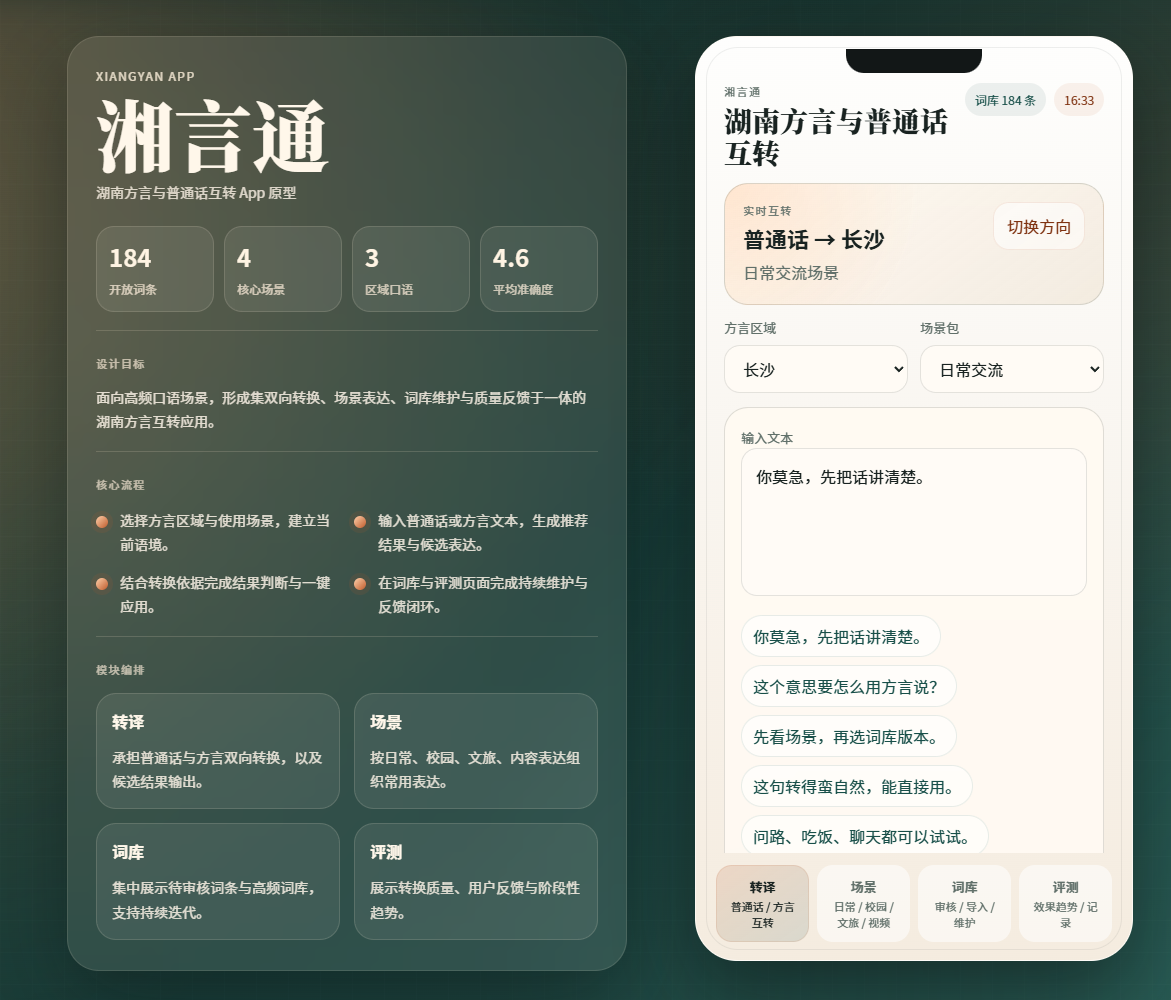
\includegraphics[width=0.8\textwidth]{APP原型首页.png}
  \caption{APP 原型首页界面}
  \label{fig:app-home}
\end{figure}

\begin{figure}[H]
  \centering
  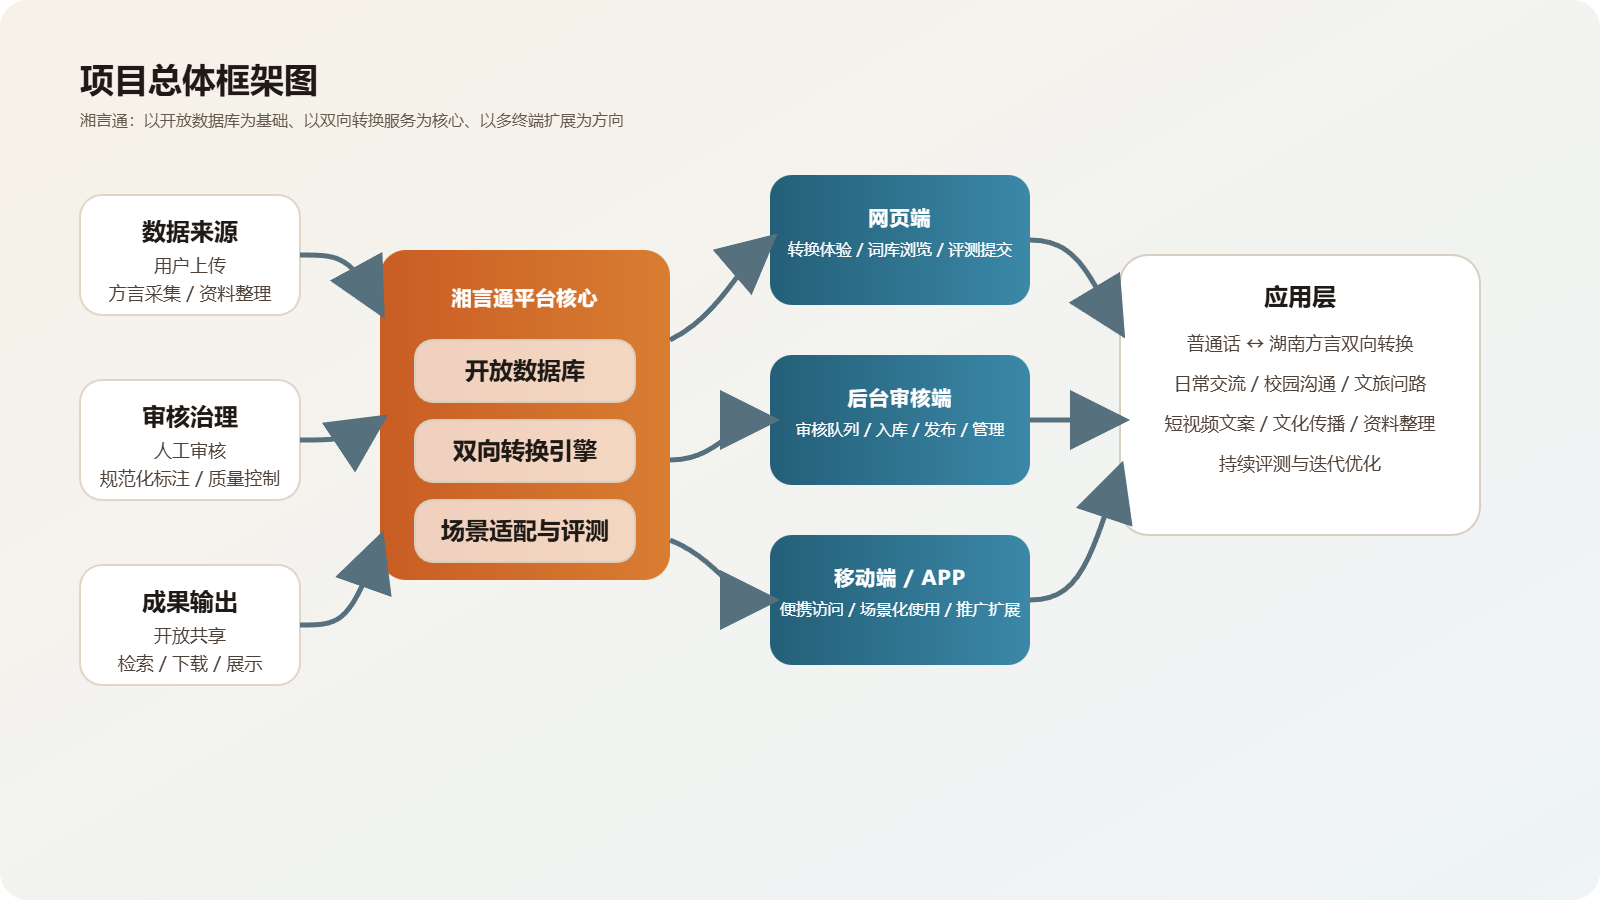
\includegraphics[width=0.8\textwidth]{项目总体框架图.png}
  \caption{项目总体框架图}
  \label{fig:framework}
\end{figure}

为说明项目已有的实现基础，现有网页平台首页界面如图~\ref{fig:web-home} 所示。该原型已能够展示方言与普通话双向转换、场景化表达、词库管理和评测反馈等内容，说明项目在功能构思和界面实现方面已完成前期探索。

\begin{figure}[H]
  \centering
  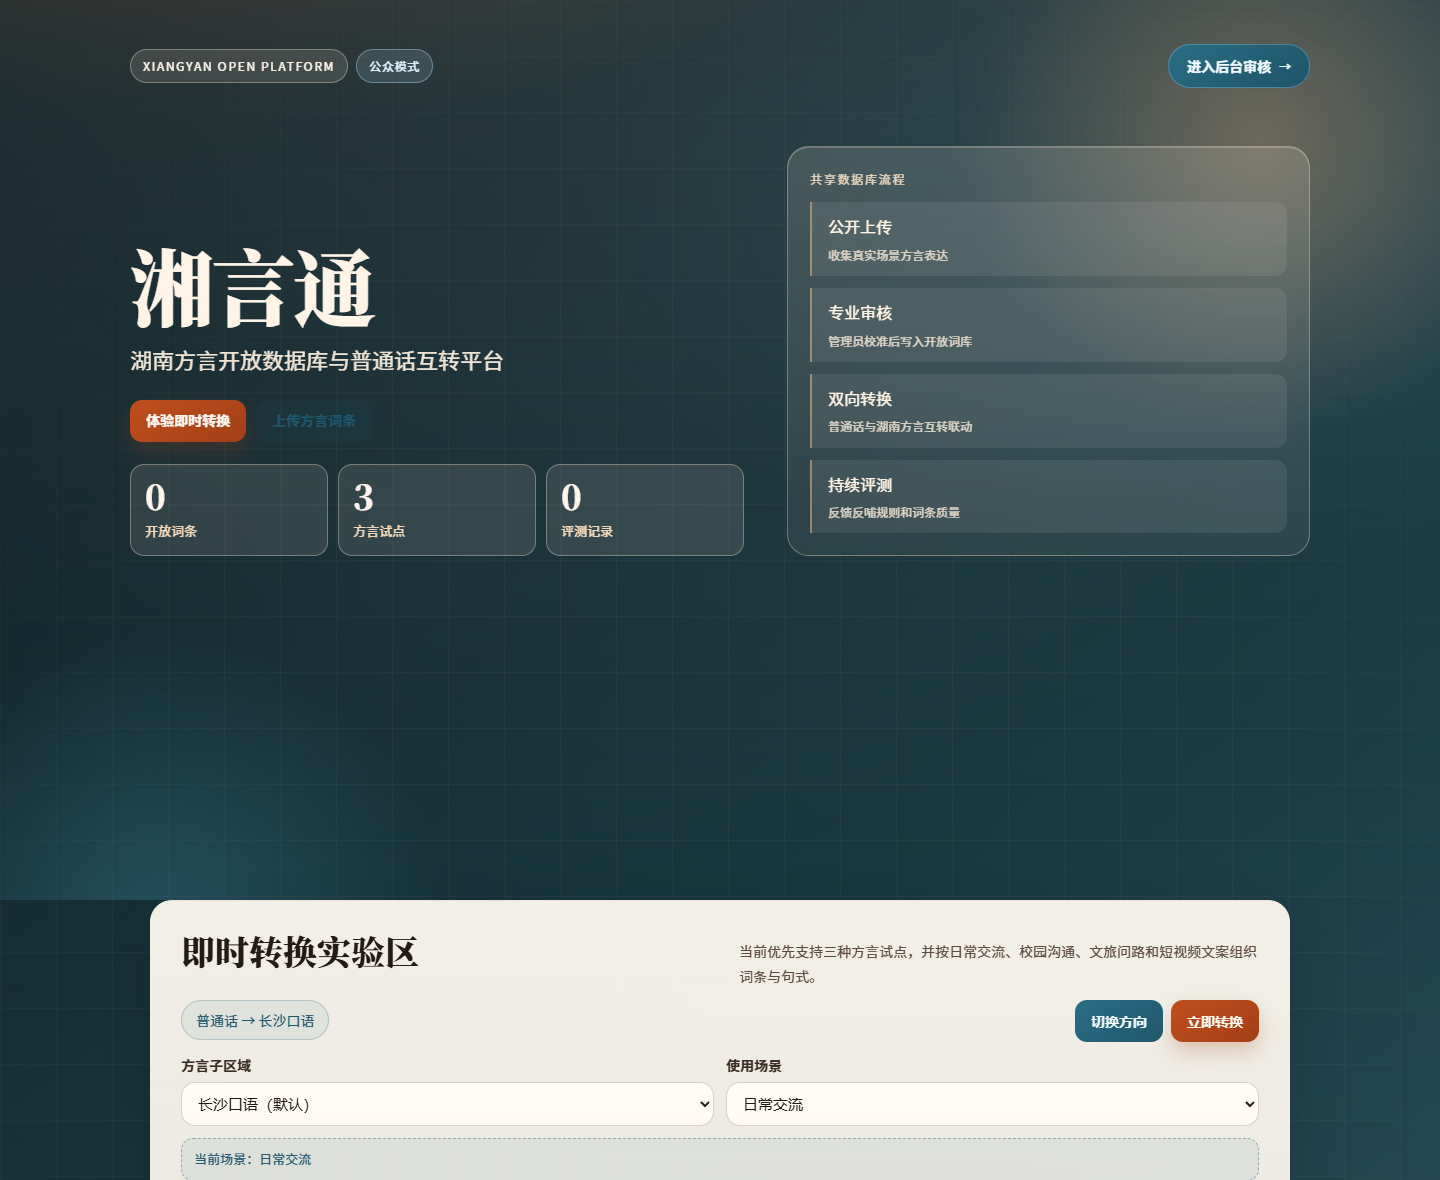
\includegraphics[width=0.8\textwidth]{湘言通首页-首屏版.png}
  \caption{湘言通网页平台首页界面}
  \label{fig:web-home}
\end{figure}

本项目的潜在使用者并不只限于土生土长的湖南方言使用者。就本地服务基础而言，湖南省统计局发布的《2024年湖南省国民经济和社会发展统计公报》显示，2024年末全省常住人口为6539万人，城镇人口为4059万人\cite{hunan2024gongbao}。湖南省政府门户网站资料显示，仅湘方言使用人口就约3085万人\cite{hunan2017fangyan}。这意味着，即便只考虑本地日常使用、方言检索和文化传播场景，项目本身就有较大的服务基础。相关数据如图~\ref{fig:local-user-data} 所示。

\begin{figure}[H]
  \centering
  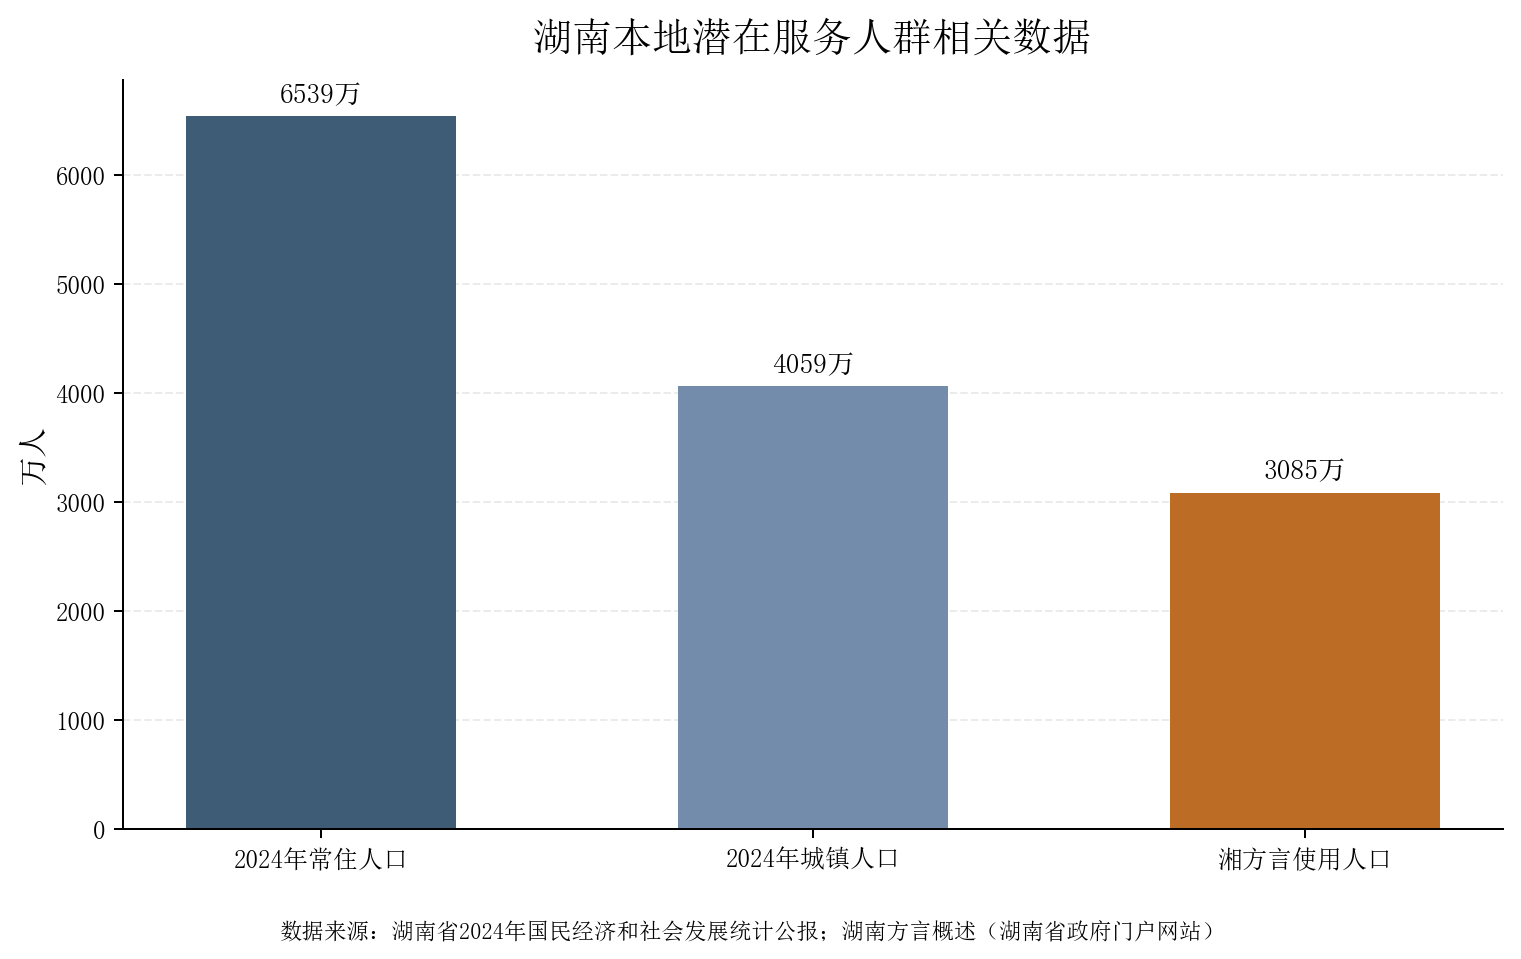
\includegraphics[width=0.8\textwidth]{hunan_local_users_chart.png}
  \caption{湖南本地潜在服务人群相关数据}
  \label{fig:local-user-data}
\end{figure}

非本地用户的需求同样存在，湖南省统计局基于第六次全国人口普查的分析指出，全省流动人口占当地常住人口比重为12.02\%，长株潭地区达到22.24\%\cite{hunanliudong2015}。这说明湖南省内跨地区流动较为明显，核心城市群的人口流动更为集中。长沙市统计局发布的《2023年长沙市国民经济和社会发展统计公报》显示，2023年末长沙市常住人口为1051.31万人，在校外来务工人员子女为19.63万人\cite{changsha2023gongbao}。这条数据虽然只是省会城市口径，但足以说明在教育、就业和城市生活场景中，外来人员与本地方言环境之间存在一定的沟通成本。对这部分人群而言，本项目可以帮助他们理解常用表达、熟悉地方语境，降低沟通成本；对本地用户而言，项目可以帮助他们检索、保存和整理熟悉却不易系统表达的方言材料。相关情况如图~\ref{fig:mobile-user-data} 和表~\ref{tab:user-groups} 所示。

\begin{figure}[H]
  \centering
  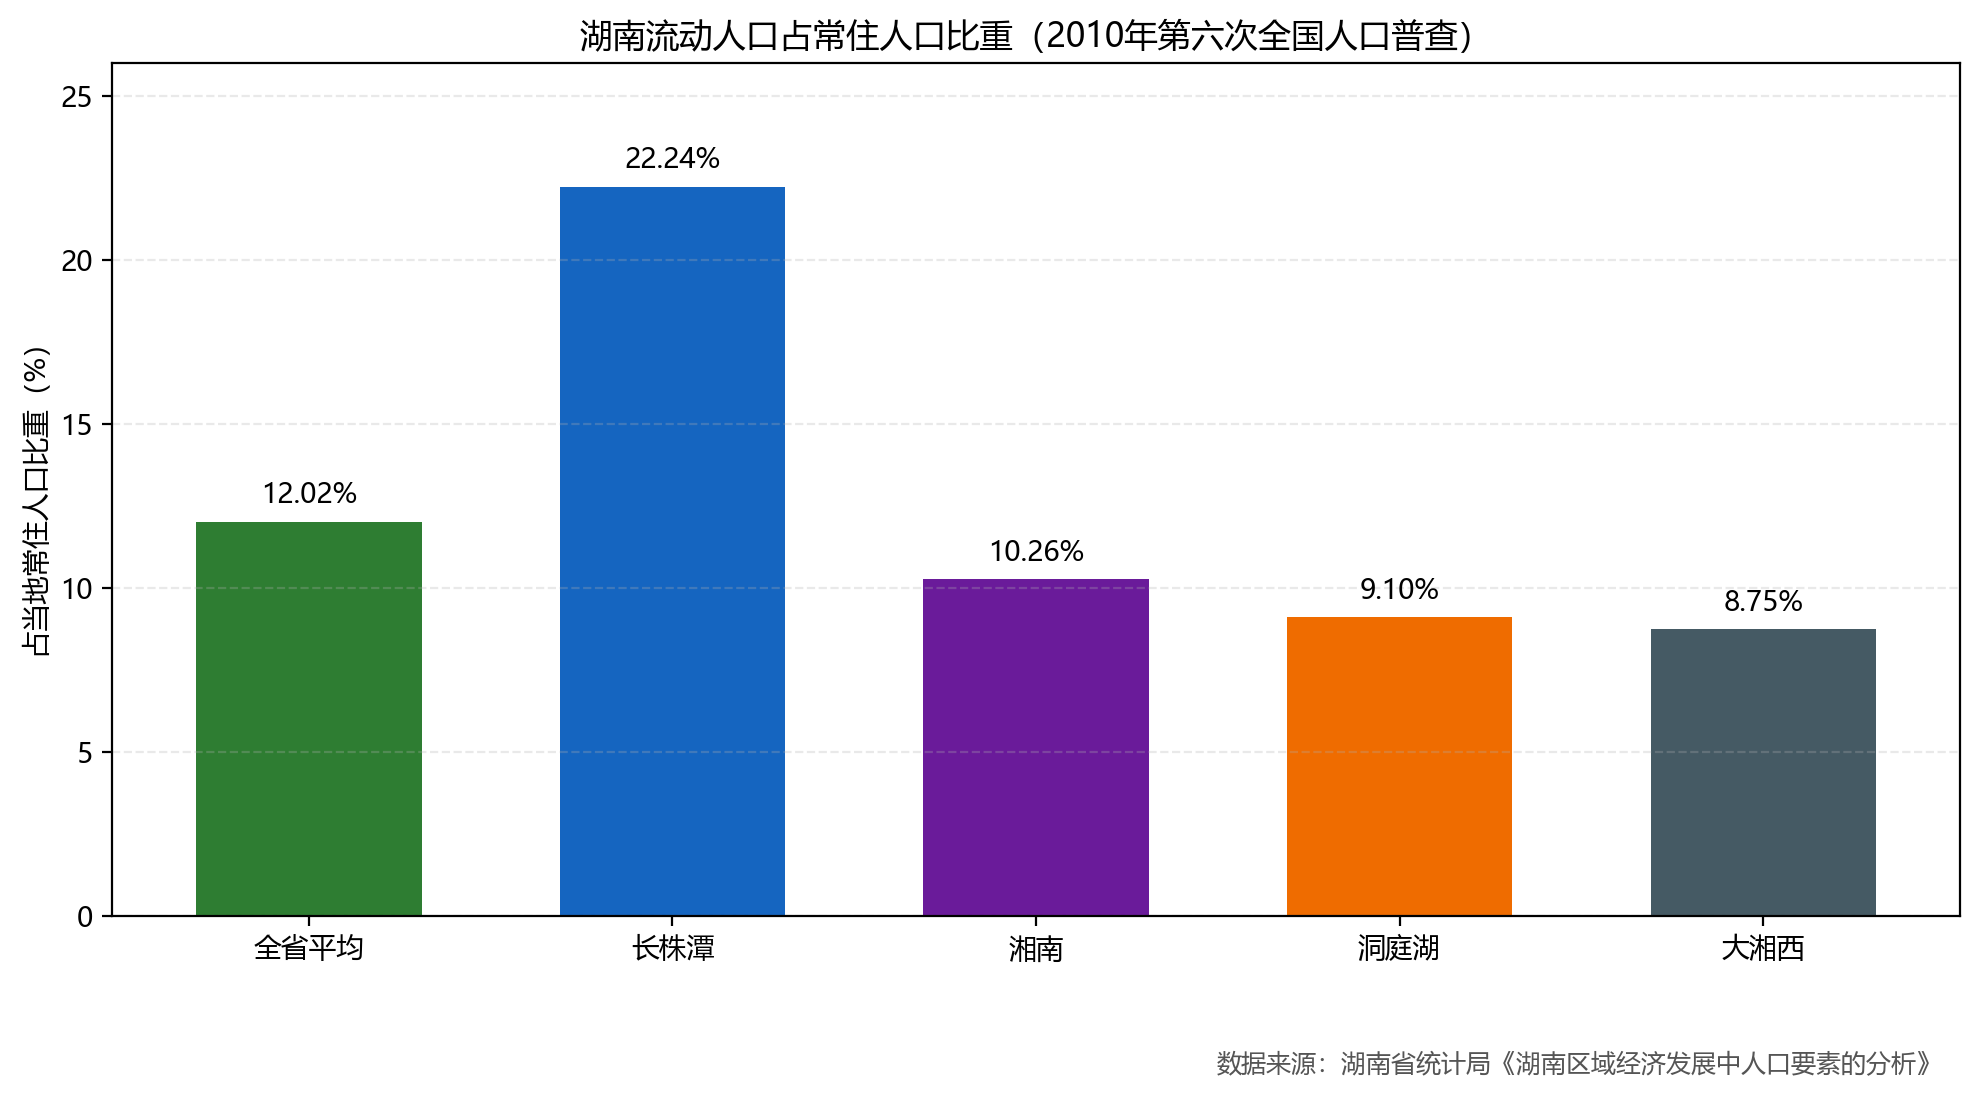
\includegraphics[width=0.8\textwidth]{湖南流动人口占比图.png}
  \caption{湖南流动人口占常住人口比重}
  \label{fig:mobile-user-data}
\end{figure}

\begin{table}[H]
  \centering
  \caption{项目潜在服务对象相关数据表}
  \label{tab:user-groups}
  \small
  \begin{tabularx}{\textwidth}{>{\raggedright\arraybackslash}p{3.1cm} >{\raggedright\arraybackslash}p{2.3cm} >{\raggedright\arraybackslash}p{2cm} Y}
    \toprule
    指标 & 数据 & 年份/口径 & 可支撑的判断 \\
    \midrule
    湖南常住人口 & 6539万人 & 2024年末 & 本地长期服务对象规模较大 \\
    湖南城镇人口 & 4059万人 & 2024年末 & 城市交流场景多，跨地区沟通需求更集中 \\
    湘方言使用人口 & 约3085万人 & 官方概述口径 & 仅湘方言就有较大的本地使用基础 \\
    长沙常住人口 & 1051.31万人 & 2023年末 & 核心城市人口集聚明显 \\
    长沙在校外来务工人员子女 & 19.63万人 & 2023年 & 外来家庭在教育场景中具有现实服务需求 \\
    湖南流动人口占常住人口比重 & 12.02\% & 第六次全国人口普查分析 & 省内跨地区流动较明显 \\
    长株潭流动人口占常住人口比重 & 22.24\% & 第六次全国人口普查分析 & 核心城市群跨地域交流需求更突出 \\
    \bottomrule
  \end{tabularx}
\end{table}

\section*{（二）研究目的}

本项目的总体目标，是面向实际使用需求，建设一个集“方言数据采集、审核整理、开放共享、双向转换和持续扩展”于一体的湖南方言数字化平台，推动地方方言资源由分散保存逐步走向规范整理、集中管理和便捷应用。研究目的既包括资源层面的积累，也包括服务层面的验证。本项目希望检验一套区域方言数字平台在小规模试点条件下能否形成稳定流程，并为后续继续扩充留下清楚的路径。

本项目主要有以下四个目标。

\begin{enumerate}
  \item 建设具有开放性和持续积累能力的湖南方言数据库。围绕词汇、短语、句式、语音样本、场景标签、释义和来源等信息，形成结构清晰、可逐步扩充的资源库，并建立基础的数据补录、修订和追踪机制。
  \item 实现普通话与湖南方言之间的双向转换。通过词汇映射、句式转换和场景适配，降低用户理解和使用湖南方言的门槛，使查询不再停留在单词对照层面。
  \item 形成便于后续扩展的平台结构。以现阶段的三种试点方言为基础，为后续继续纳入更多方言点、增加语音功能和开发移动端应用预留空间，避免后续扩展时重复改动底层结构。
  \item 探索“数据库建设 + 语言服务平台 + 移动端延伸”相结合的实现路径，使方言保护工作由静态保存进一步走向动态服务和持续应用，并为高校团队后续持续维护提供可执行的范式。
\end{enumerate}

为使研究目标更加清晰明确，现将本项目的总体目标细化为表~\ref{tab:goals}所示的若干子目标。需要强调的是，这些目标并非彼此孤立、相互割裂，而是相互支撑、协同推进的有机整体：数据库建设关系到平台能否持续积累与更新内容，转换功能决定平台是否具备实际应用价值，审核与反馈机制影响结果的可靠性与可信度，而多终端扩展则关系到项目能否实现进一步的推广与应用。

\begin{table}[H]
  \centering
  \caption{项目目标分解}
  \label{tab:goals}
  \small
  \begin{tabularx}{\textwidth}{>{\raggedright\arraybackslash}p{2.6cm} Y Y}
    \toprule
    目标维度 & 核心任务 & 预期效果 \\
    \midrule
    数据资源建设 & 构建涵盖方言词汇、句式、语音及场景标签的结构化数据库 & 形成可持续积累与动态更新的基础数据资源体系 \\
    平台功能建设 & 实现普通话与方言的双向转换功能，并支持词条上传、审核与检索等核心模块 & 提升平台整体服务能力与实际应用价值 \\
    质量保障建设 & 构建后台审核机制与评测反馈体系，实现数据与结果的持续校验与优化 & 提高数据可靠性与转换结果的可信度 \\
    应用拓展建设 & 推进多方言扩展，开展语音模块预研，并探索 APP 原型开发与功能延伸 & 增强项目的推广潜力与长期发展能力 \\
    \bottomrule
  \end{tabularx}
\end{table}

\section*{（三）研究内容}

本项目的研究内容主要包括以下四个方面。这四部分在实际实施过程中彼此关联、相互影响：数据库设计直接关系到转换效果，而具体的转换需求又会反过来推动字段设计与样本补充的完善；多终端应用的引入，则能够在实际使用中检验平台在交互方式与数据组织方面存在的问题。因此，尽管研究内容在结构上分为若干部分展开，但在推进过程中将采取边建设、边调整、逐步完善的实施方式。

\subsection*{1. 开放方言数据库建设与管理机制研究}

这部分主要围绕湖南方言的词汇、常用短语、句式表达、语音样本以及相关的场景标签、释义说明、来源信息和审核状态等内容，设计一套结构清晰的数据组织方式，并据此建立支持上传、审核、入库、检索与导出的数据库管理机制。数据来源既包括用户提交与实地整理所得的材料，也涵盖专业词典、方言研究著作及地方文献等相对稳定的书面资料。平台拟采用“多来源采集—后台审核—结构化入库”的基本流程，在保持数据开放性的同时，尽量确保其可靠性与规范性。需要说明的是，这里的“数据库建设”并不仅是简单的数据汇集，更重要的是形成一套可持续执行的整理规则，例如同义表达的归并策略、异形词的处理方式、来源可信度的标注规范以及审核过程的记录机制。数据库建设的基本流程如图~\ref{fig:database-flow} 所示。

在具体实施过程中，需要重点处理几类常见情况：其一，同一词语在不同地区可能存在不同写法；其二，相同表达在不同语境中的含义并不完全一致；其三，书面文献与口述材料之间可能存在差异。针对这些问题，数据库不采用单一“标准答案”的处理方式，而是尽量保留地区信息、来源信息以及必要的释义说明。虽然这会增加整理工作的复杂度，但有助于更真实地呈现方言本身的差异性，避免对其进行过度简化。

\begin{figure}[H]
  \centering
  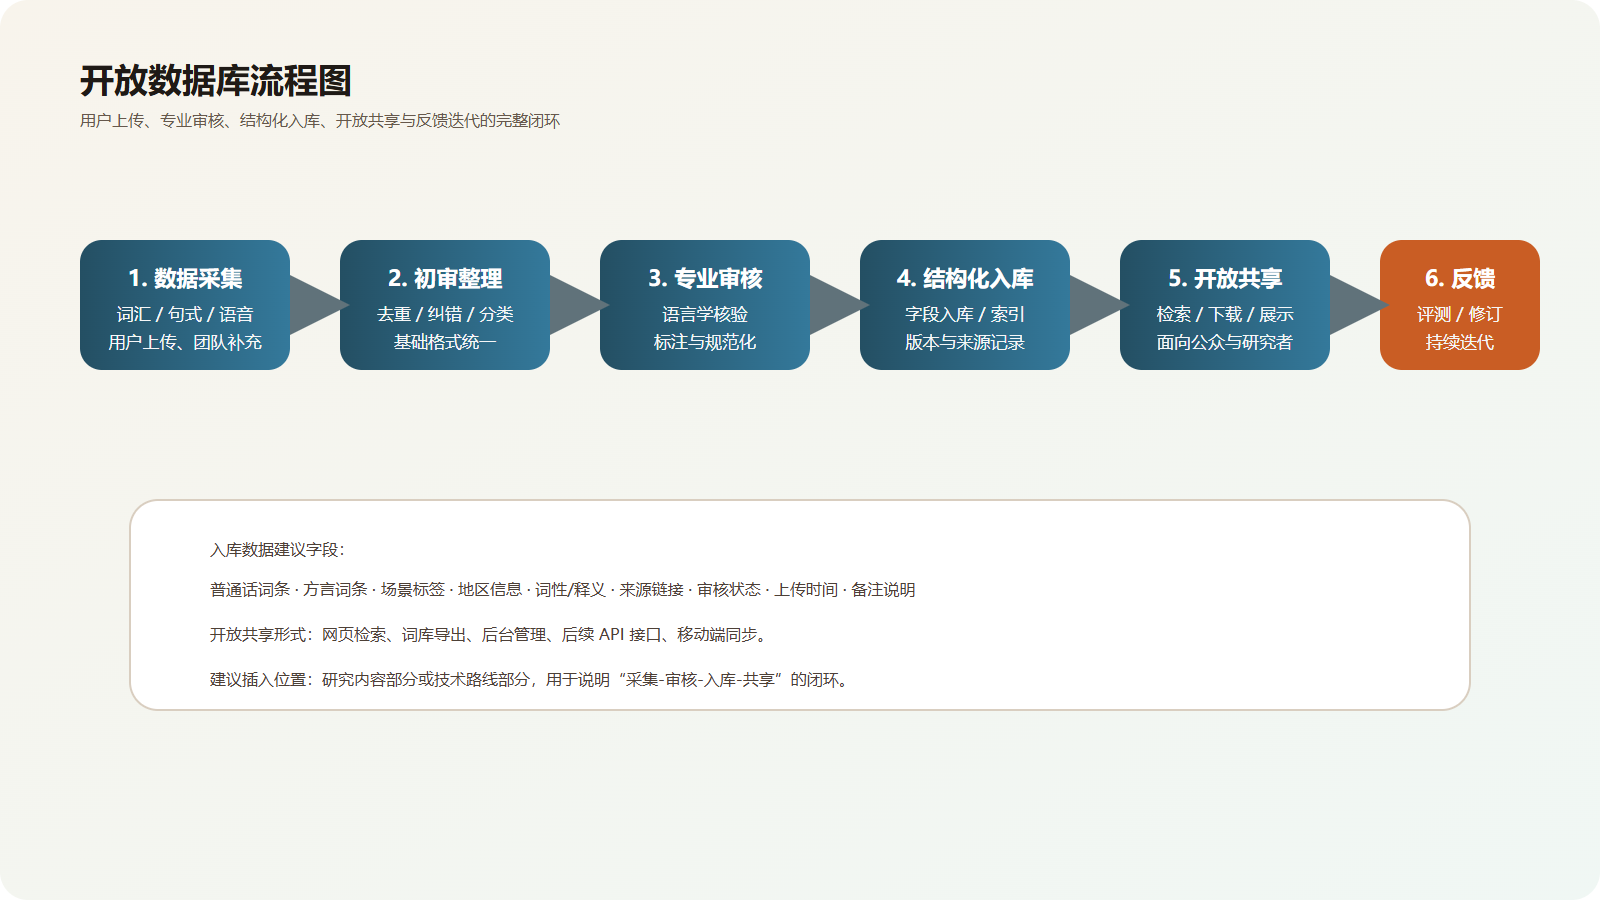
\includegraphics[width=0.8\textwidth]{开放数据库流程图.png}
  \caption{开放数据库建设流程图}
  \label{fig:database-flow}
\end{figure}

为提高数据库设计的规范性与一致性，本项目拟采用表~\ref{tab:fields} 所示的核心字段结构。字段设置在保持简洁的前提下，兼顾关键信息的完整表达。其中，“来源”和“审核状态”两项尤为关键，它们直接影响数据是否具备进一步引用与扩展的基础。

\begin{table}[H]
  \centering
  \caption{数据库核心字段设计表}
  \label{tab:fields}
  \small
  \begin{tabularx}{\textwidth}{>{\raggedright\arraybackslash}p{2.2cm} >{\raggedright\arraybackslash}p{3.6cm} >{\raggedright\arraybackslash}p{2cm} Y}
    \toprule
    字段名 & 含义 & 是否必填 & 示例 \\
    \midrule
    普通话词 & 标准汉语词条 & 是 & 漂亮 \\
    方言词 & 对应湖南方言表达 & 是 & 标致 \\
    方言点 & 所属区域或口音点 & 是 & 长沙 \\
    场景标签 & 使用场景分类 & 否 & 日常交流 \\
    释义 & 词义说明 & 否 & 外貌好看 \\
    来源 & 数据采集来源 & 否 & 用户上传/调查/专业词典/文献 \\
    审核状态 & 当前审核状态 & 是 & 待审/通过/驳回 \\
    \bottomrule
  \end{tabularx}
\end{table}

\subsection*{2. 方言与普通话双向转换功能研究}

这部分围绕普通话转方言和方言转普通话两个方向开展研究，重点处理词汇对应、句式转换、语义近似表达以及场景适配等问题。由于方言表达具有明显的地域差异和语境依赖，转换过程不能仅依赖简单的词典替换，还需要结合常见使用场景、候选表达以及解释反馈，对结果进行综合调整。已有研究表明，低资源语言或方言相关技术通常需要先建立相对稳定的数据基础，再逐步完善转换与评测机制\cite{lau2022wordshk,yu2022asr,suen2024pivot}，这一思路与本项目当前阶段的安排基本一致。

在实现路径上，更侧重于结果的可用性。现阶段不以复杂模型为重点，而是优先完善高频词汇、常用句式、典型场景以及解释反馈等基础内容。对于难以做到严格一一对应的表达，不强求给出唯一结果，而是提供若干候选表达及其适用说明。这种处理方式更符合方言转换的实际情况，也有助于在使用过程中逐步积累优化所需的数据与反馈。

\subsection*{3. 多方言接入与功能扩展研究}

目前，项目优先选取长沙、湘潭、株洲三地作为试点方言点，在此基础上构建具备良好扩展性的数据库模型与功能模块，为后续接入更多湖南方言提供统一且稳定的技术框架。之所以采取分阶段试点策略，是因为区域性方言平台若在初期盲目扩大覆盖范围，往往容易导致样本分布不均、审核机制滞后以及字段标准频繁调整等问题。通过在较小范围内先行打通整体流程，有助于在实践中不断校准规范，从而为后续稳步扩展奠定坚实基础。

同时，项目在系统架构层面预留语音转换与语音互转（speech-to-speech）等扩展接口，以满足未来由“文本服务”向“文本 + 语音服务”演进的需求。现阶段的核心目标并非追求复杂算法的快速落地，而是着力提升资源组织方式、字段规范体系及扩展机制的稳定性与一致性。扩展研究的重点在于：确保在新增方言点时，无需推翻既有数据结构，也无需对平台的审核流程与展示逻辑进行大规模重构，从而实现系统的平滑演进与长期可持续发展。

\subsection*{4. 多终端应用与推广场景研究}

本项目将在现有网页原型基础上，进一步优化交互流程、数据管理方式与展示逻辑，并结合移动端使用场景推进 APP 化原型研究，使系统更契合手机用户在日常交流、文旅传播、学习理解及资料整理等高频场景中的使用需求。已有语言资源平台的实践表明，资源建设若要真正形成良好的实际应用效果，往往还需要配合清晰的展示逻辑与明确的服务入口\cite{guojiafuwu,zhongguocaolu,zhongguowenzi}。

这一部分不仅是界面适配问题，也关系到平台的实际使用频率。网页端更适合资料整理、后台审核与集中展示，移动端更适合查询、比对、收藏和轻量上传。区分不同终端的使用任务，有助于明确平台定位，并符合用户的实际使用习惯。
在此基础上，项目将通过模块化设计优化功能结构，在不改变既有参考文献与图表的前提下，提高系统的可扩展性与使用效率。

\section*{（四）国内外研究现状和发展动态}

\subsection*{1. 国内研究现状}

国内关于汉语方言的研究，已经从早期以语音、词汇、声调和方言分区为主，逐步拓展到语言生态、社会认同、资源保护以及数字化整理等方向\cite{cao2015dingwei,liru2001fangyanxue,yuanjia2021gaibao,shilin2017shengtai}。尤其是中国语言资源保护工程的持续推进，表明我国在方言及地方语言资源的记录、整理、保存、展示和开发利用等方面，已逐渐形成较为系统的工作体系\cite{jiaoyubu2024baohu,cao2015dingwei}，为本项目提供了清晰的研究背景和方法参考。

从已有成果来看，国内在资源采集、方言档案建设、调查资料整理以及展示平台搭建等方面，已经积累了较为丰富的经验，这些成果为本项目提供了重要借鉴。但针对某一具体地区，同时兼顾资源库建设、服务入口和持续补充机制的平台仍相对较少。现有研究多侧重于资料保存、成果发布或集中展示，在交互功能、公众参与以及持续更新等方面，还有进一步完善的空间。
国家语言资源服务平台、中国语言资源采录展示平台和中国语言文字数字博物馆等，已经体现出“资源采集—成果展示—公共传播—服务整合”相结合的发展趋势，说明语言资源建设正由单一保存逐步转向“保存 + 展示 + 服务”的综合模式。相关平台示例如图~\ref{fig:national-platform}、图~\ref{fig:collection-platform} 和图~\ref{fig:digital-museum} 所示。

\begin{figure}[H]
  \centering
  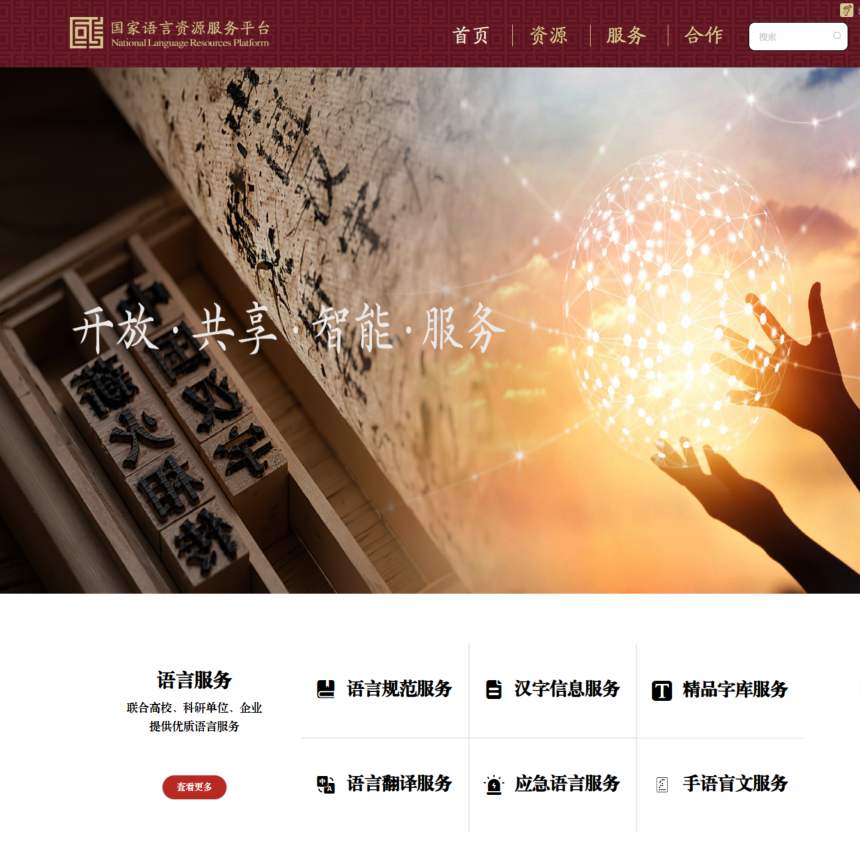
\includegraphics[width=0.8\textwidth]{国家语言资源服务平台.png}
  \caption{国家语言资源服务平台首页}
  \label{fig:national-platform}
\end{figure}

\begin{figure}[H]
  \centering
  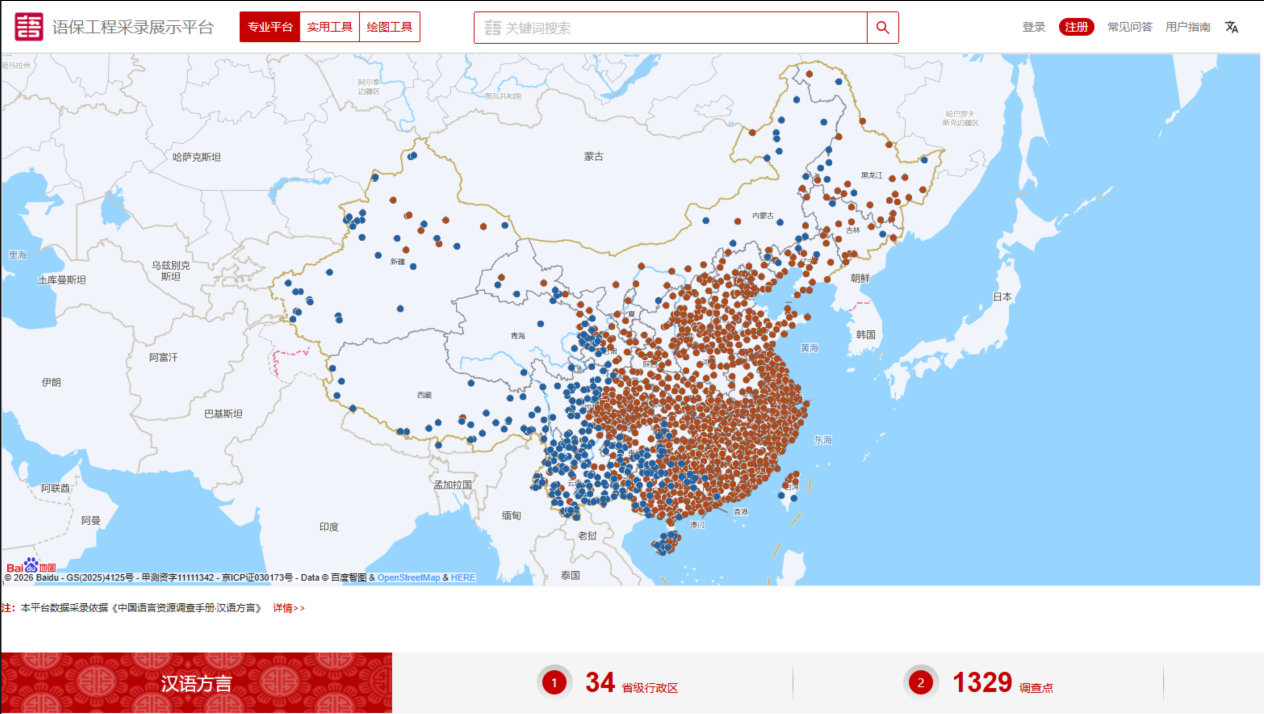
\includegraphics[width=0.8\textwidth]{中国语言资源采录展示平台.png}
  \caption{中国语言资源采录展示平台首页}
  \label{fig:collection-platform}
\end{figure}

\begin{figure}[H]
  \centering
  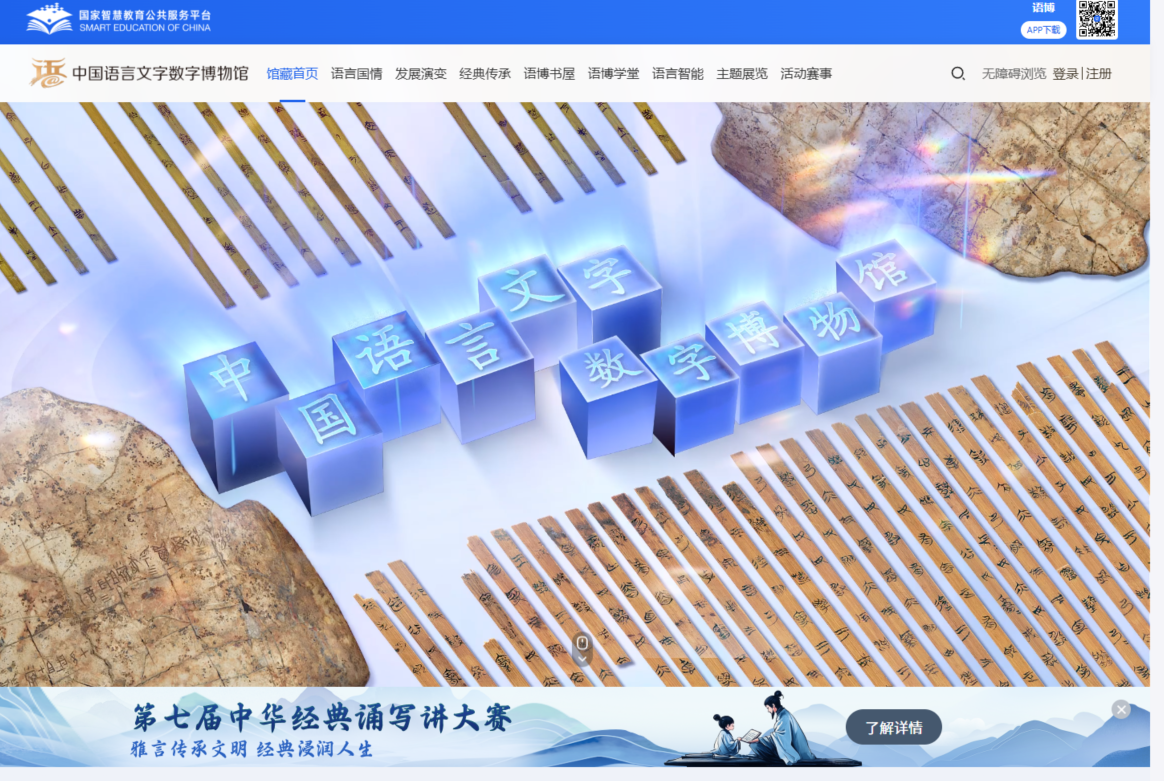
\includegraphics[width=0.8\textwidth]{中国语言文字数字博物馆.png}
  \caption{中国语言文字数字博物馆首页}
  \label{fig:digital-museum}
\end{figure}

\subsection*{2. 国外研究现状}

国际上关于低资源语言和方言技术的研究，主要关注在数据有限的情况下，如何开展资源建设、明确任务类型、建立基础系统并逐步优化\cite{lau2022wordshk,yu2022asr,suen2024pivot}。无论是词典类数据集、语音识别数据集，还是方言翻译系统，多数研究都表明，数据资源的建设是后续算法开发和应用服务的基础。国外相关研究的一个显著特点，是对元数据、版本信息以及使用场景说明更加重视，这一点对本项目具有直接参考意义。

在平台建设方面，PARADISEC、ELAR、The Language Archive 等国际语言资源平台，普遍重视长期保存、元数据管理、资源检索以及共享机制。这类平台更强调资源整理的规范性和长期可用性，其服务对象也多以研究和档案使用为主。对本项目而言，这些经验的价值不在于直接复制平台形式，而在于借鉴其资源描述方法、归档思路和共享规则。其中，PARADISEC 平台如图~\ref{fig:paradisec} 所示。

\begin{figure}[H]
  \centering
  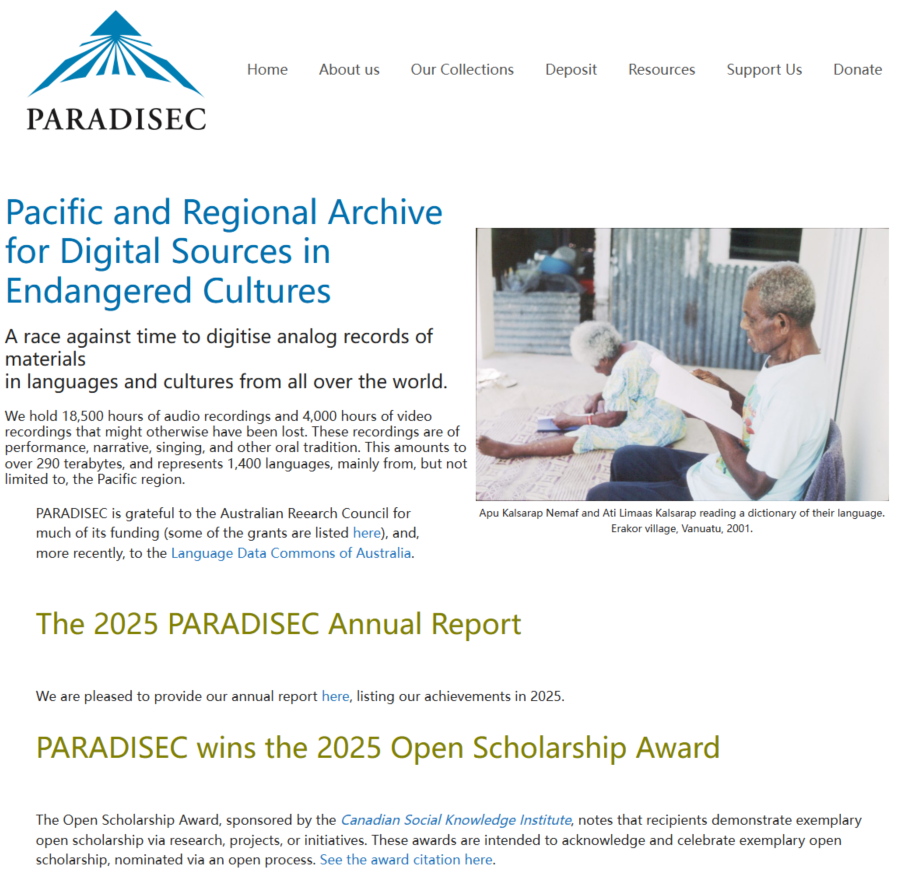
\includegraphics[width=0.8\textwidth]{PARADISEC.png}
  \caption{PARADISEC 平台首页}
  \label{fig:paradisec}
\end{figure}

\subsection*{3. 现有研究的不足}

现有研究和相关平台仍存在以下几方面不足：

\begin{enumerate}
  \item 许多研究仍以单一方向为主，例如只建设词典、只开展语音识别或只实现句子翻译，缺少将“采集、审核、入库、转换、评测、迭代”等环节贯通起来的完整流程。
  \item 面向湖南方言的公开数据资源、统一标注规范、多方言扩展机制以及与普通话的双向转换基础仍不够完善。
  \item 同时兼顾数据库建设、公众服务与移动端应用的综合型平台仍较为有限，区域方言的数字化服务能力仍有提升空间。
\end{enumerate}

这些不足并不意味着已有工作不充分，而是反映出不同研究在目标和使用场景上的侧重点存在差异。部分项目更偏重档案保存，部分侧重调查记录或成果展示，而本项目则尝试将资料积累、转换服务与持续维护整合在同一平台中加以考虑。为使现状分析更加直观，可将典型平台与本项目的关系整理为表~\ref{tab:comparison}。

\begin{table}[H]
  \centering
  \caption{相关平台与本项目对比表}
  \label{tab:comparison}
  \small
  \begin{tabularx}{\textwidth}{>{\raggedright\arraybackslash}p{2.2cm} >{\raggedright\arraybackslash}p{2.5cm} >{\raggedright\arraybackslash}p{2.7cm} >{\raggedright\arraybackslash}p{2.3cm} Y}
    \toprule
    平台/项目 & 主要特点 & 现有优势 & 局限性 & 对本项目的启示 \\
    \midrule
    国家语言资源服务平台 & 资源服务聚合 & 国家级、权威性高、服务导向明显 & 地方方言定制化不强 & 借鉴“资源库 + 服务平台”一体化思路 \\
    中国语言资源采录展示平台 & 采录与展示结合 & 贴近采集、展示、检索链路 & 偏展示型，转换服务有限 & 借鉴采录展示和结构化入库机制 \\
    中国语言文字数字博物馆 & 公共传播与数字展示 & 多模态、适合文化传播 & 语言服务属性相对较弱 & 借鉴数字展示和传播方式 \\
    PARADISEC & 国际语言档案平台 & 长期保存、元数据规范 & 本土应用场景较远 & 借鉴归档、分类和共享模式 \\
    湘言通 & 湖南方言数据库与转换平台 & 兼顾数据库、转换、审核和扩展 & 仍处于建设完善阶段 & 形成区域方言平台化综合方案 \\
    \bottomrule
  \end{tabularx}
\end{table}

\subsection*{4. 本项目的切入点}

在上述研究基础上，本项目立足湖南方言的实际使用场景，将资源整理、平台建设与转换服务结合推进。项目的重点不在于单一算法的展示，而在于通过开放数据库促进资源积累，通过双向转换满足实际使用需求，通过后台审核与评测反馈提升平台质量，并在此基础上逐步向移动端延伸。与单纯展示型平台相比，本项目更强调“可积累、可维护、可扩展、可使用”。

这一思路也决定了项目不会将重心放在“展示效果”上。网页和 APP 原型固然重要，但它们主要是资源组织和服务逻辑的呈现形式。真正影响项目质量的，是数据能否持续进入系统、审核机制能否稳定运行、用户能否获得较为可靠的转换结果，以及项目结束后平台是否具备持续维护和更新的能力。

\section*{（五）创新点与项目特色}

本项目的主要特色和创新点可概括为以下几个方面。这些特点并不在于提出全新的理论，而在于将区域方言平台中常见的几个分散问题放入一个可落地的整体框架中加以解决。

\begin{enumerate}
  \item 以开放数据库建设为核心。项目不仅用于展示内容，还致力于构建一个可持续积累、可审核、可共享的湖南方言资源库，使资料的补充、筛选与修订能够在同一体系内完成。
  \item 以双向转换为主要应用场景。将普通话与湖南方言之间的转换需求整合到同一平台中，提升实际使用价值，同时也为数据库建设提供明确的应用方向。
  \item 通过“用户上传 + 后台审核 + 评测反馈”形成完整流程。在鼓励用户参与的同时，加强质量控制与持续优化，避免内容在扩展过程中出现偏差。
  \item 以多终端支持和后续扩展为发展方向。在保留网页端展示与管理功能的基础上，为多方言接入及语音转换预留接口，增强系统的延展能力，减少后续扩展时的重复开发。
\end{enumerate}

此外，湖南本地已开展一定的方言文化资源开发实践，这从侧面说明本项目具备良好的区域基础和现实可行性。相比完全依赖外部案例，这种本地实践更有利于后续开展资源采集、展示与传播工作。地方实践案例如图~\ref{fig:hunan-news} 所示。

\begin{figure}[H]
  \centering
  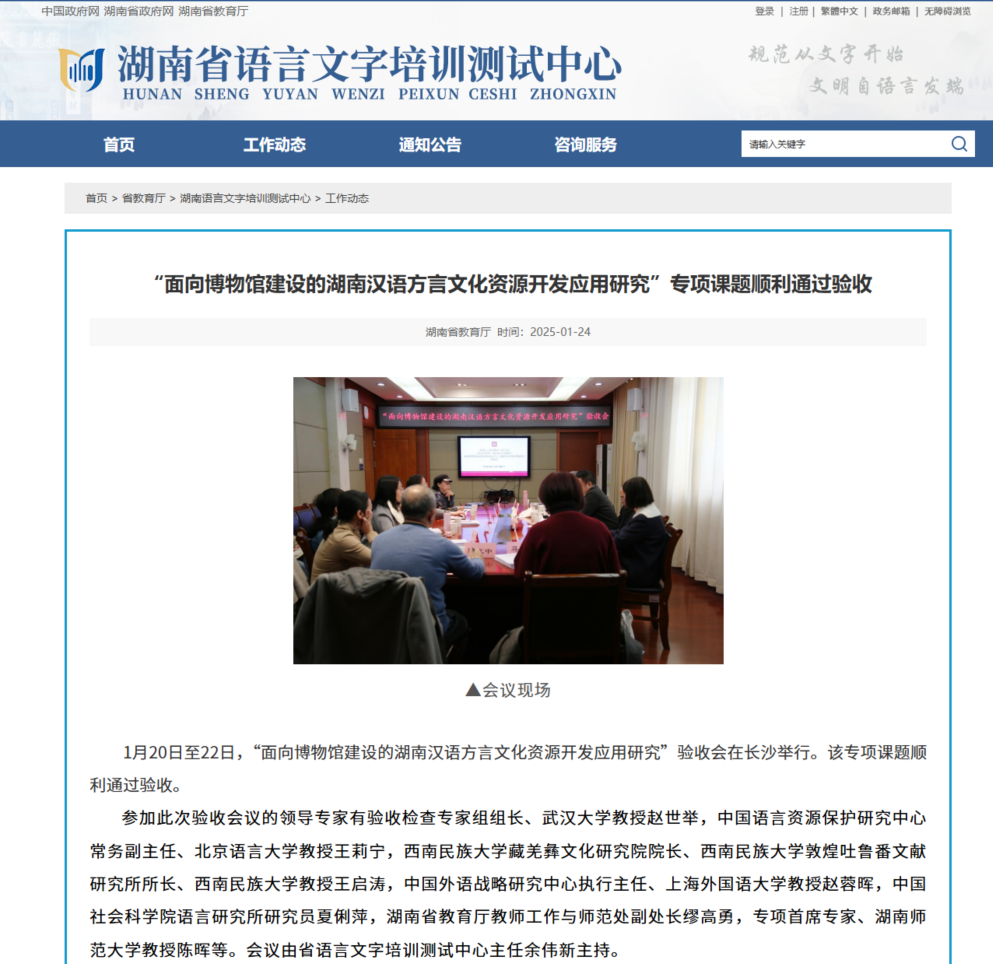
\includegraphics[width=0.8\textwidth]{湖南方言文化资源开发应用研究新闻页.png}
  \caption{湖南省教育厅方言资源开发应用研究新闻页}
  \label{fig:hunan-news}
\end{figure}

\section*{（六）技术路线、拟解决的问题及预期成果}

\subsection*{1. 技术路线}

本项目拟按照“平台原型完善—数据库结构设计—数据采集上传—专业审核入库—双向转换优化—多终端拓展”的技术路线推进实施。整体技术路线如图~\ref{fig:tech-roadmap} 所示。其核心思路是优先打牢底层数据与流程基础，再逐步完善展示功能与使用场景，避免因追求界面效果或功能叠加而频繁调整数据结构。

\begin{figure}[H]
  \centering
  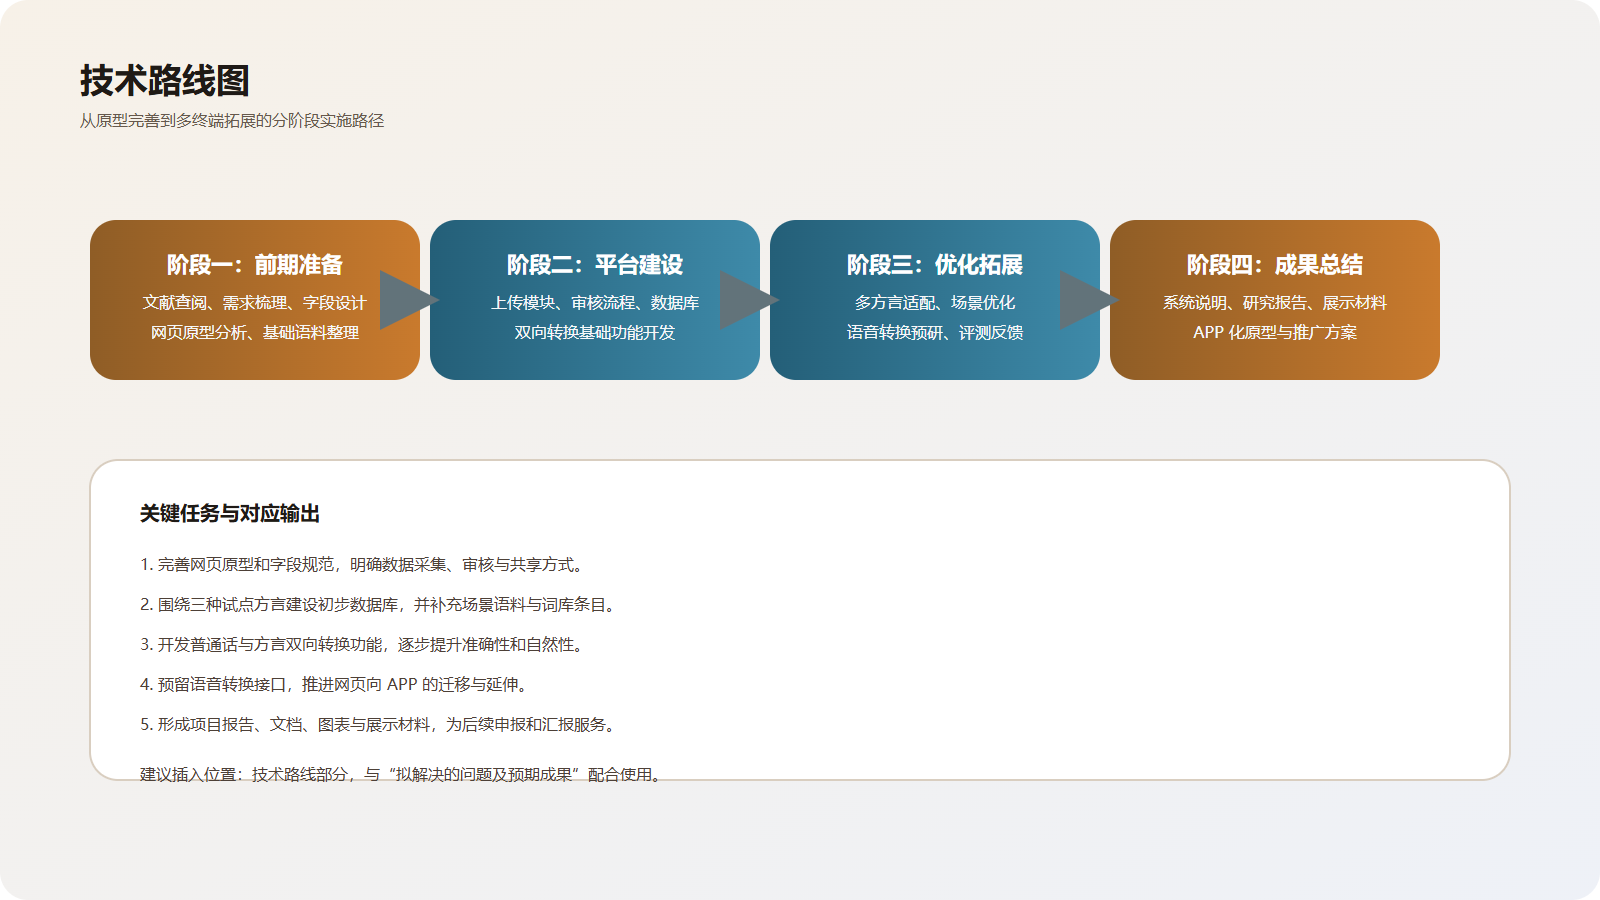
\includegraphics[width=0.8\textwidth]{技术路线图.png}
  \caption{技术路线图}
  \label{fig:tech-roadmap}
\end{figure}

具体内容如下：

\begin{enumerate}
  \item 在现有网页原型基础上，进一步完善系统架构与交互逻辑，明确字段规范、上传规范、审核流程和共享方式。
  \item 围绕三类试点方言，整理基础语料与常见表达，建设初步数据库，并同步检验字段设计是否符合实际使用需求。
  \item 开发并优化普通话与方言之间的双向转换功能，提升系统在实际场景中的可用性，逐步补充高频表达及其说明信息。
  \item 预留语音转换模块接口，为后续实现方言与普通话之间的语音互转做好准备，使文本服务与语音服务能够顺利衔接。
  \item 结合移动端使用需求，推进 APP 原型研究与后续拓展，形成更适合日常查询和轻量使用的服务形态。
\end{enumerate}

该技术路线的优点在于各阶段目标清晰、成果可见。即使后续扩展尚未完全展开，前期形成的数据库、网页平台及试点方言样本，仍可作为阶段性成果加以保留和使用。

\subsection*{2. 拟解决的问题}
本项目拟重点解决表~\ref{tab:issues} 所示问题。总体来看，主要集中在“资料收集困难、数据管理不规范、转换功能不完善、平台持续性不足”四个方面。

\begin{table}[H]
  \centering
  \caption{拟解决问题与对应方案表}
  \label{tab:issues}
  \small
  \begin{tabularx}{\textwidth}{>{\raggedright\arraybackslash}p{2.3cm} >{\raggedright\arraybackslash}p{3cm} >{\raggedright\arraybackslash}p{3cm} Y}
    \toprule
    现存问题 & 问题表现 & 对应方案 & 预期效果 \\
    \midrule
    方言资源分散 & 数据来源零散、难以集中整理 & 建设统一上传与入库平台 & 提高数据积累效率 \\
    数据缺乏规范 & 字段不统一、来源不清晰 & 建立审核机制和字段标准 & 提高数据可用性与可信度 \\
    转换工具功能单一 & 仅用于展示，缺少实际应用功能 & 构建双向转换、评测反馈和候选解释 & 提升平台服务能力 \\
    移动端应用不足 & 网页端难以覆盖高频使用场景 & 推进 APP 原型和移动端适配 & 提高项目使用率与传播效果 \\
    \bottomrule
  \end{tabularx}
\end{table}

\subsection*{3. 预期成果}

本项目的预期成果主要包括：

\begin{enumerate}
  \item 构建一个较为完整的湖南方言与普通话双向转换网页平台，支持查询、展示、上传、审核及基础转换等功能。
  \item 建设一个支持用户上传、专业审核与开放共享的方言数据库，形成可持续扩展的基础资源库。
  \item 完成三类试点方言的数据整理与接入，形成具有代表性的样本与常见表达集合。
  \item 形成语音转换功能的初步设计方案与扩展接口，为后续开发预留基础。
  \item 完成由网页向 APP 延伸的原型方案，使项目具备向移动端发展的条件。
  \item 形成项目研究报告、系统说明文档及相关展示材料，为后续申报与持续研究提供支撑。
\end{enumerate}

上述成果既包括可直接展示和使用的平台与原型，也包括数据库结构、审核规则及文档材料等基础内容。两者相互支撑：前者提升使用体验，后者保证系统能够长期稳定运行。

\section*{（七）项目研究进度安排}
项目研究拟分四个阶段推进，具体安排如表~\ref{tab:schedule} 所示。整体进度遵循“先整理、再建设、再优化、再总结”的顺序，每一阶段均对应明确成果，避免仅有时间安排而缺乏实际产出。

\begin{table}[H]
  \centering
  \caption{项目研究进度安排表}
  \label{tab:schedule}
  \small
  \begin{tabularx}{\textwidth}{>{\raggedright\arraybackslash}p{3.2cm} Y Y}
    \toprule
    阶段 & 主要任务 & 阶段成果 \\
    \midrule
    第一阶段：前期准备与资料整理 & 完成文献查阅、需求梳理、字段设计、网页原型分析以及三类方言基础语料的初步整理 & 需求分析文档、字段设计文档、基础语料清单 \\
    第二阶段：平台建设与功能开发 & 完善数据上传、后台审核、数据库管理及双向转换等核心功能模块 & 可运行的网页平台、初步数据库、审核流程 \\
    第三阶段：优化与拓展 & 优化多方言适配效果、转换质量、共享机制与用户体验，推进语音功能预研及 APP 原型完善 & 优化后的平台、扩展方案、APP 原型 \\
    第四阶段：总结与提升 & 完成研究报告、系统说明及展示材料，总结项目经验与存在问题 & 结题材料、展示文档、项目总结报告 \\
    \bottomrule
  \end{tabularx}
\end{table}

\section*{（八）已有基础}

本项目已具备一定的前期基础。团队已完成网页原型的初步搭建，并实现了可展示的方言与普通话双向转换页面，表明在功能设计和界面实现方面已取得阶段性进展。围绕方言与普通话的转换需求，团队也已开始整理相关词汇与表达，对平台的数据组织方式、功能结构及使用场景形成了初步认识。现有原型虽仍需完善，但已能够支持对主要功能模块进行拆分与验证，而非从零起步。

项目同时具备向 APP 延伸的思路与原型基础。当前 APP 原型地址为 \url{https://courageous-conkies-6dd293.netlify.app/}，可为后续移动端开发提供参考。网页原型与 APP 原型之间的对应关系，也有助于提前识别不同终端在功能层级与交互重点上的差异。
此外，湖南本地已有一定的方言文化资源开发与展示实践，这表明本项目具备良好的区域基础和推进条件。目前，项目在原型设计、功能方向、研究主题及应用场景等方面已形成较为清晰的前期准备。后续工作的重点在于扩充数据来源、完善审核规范、提升多方言适配能力，并逐步推进语音功能与移动端拓展。总体来看，团队已具备开展本项目的基础条件，下一步关键在于将已有设想进一步细化并稳定落实。

\printbibliography[title={参考文献}]

\end{document}
